\section{Leak Tests using Spectroscopy}
Once the cell is sealed and activated with the alkali metal 
vapor (typically Rb or Cs), leak tests can be performed over 
time to estimate its hermeticity. Leak tests 
involving laser absorption spectroscopy have been
reported in literature 
\cite{pitz2009, pitz2010, andalkar2002, pitz2014, shi2019}.
 In these tests, a tunable laser 
interacts with the alkali atoms. By measuring the width and 
central frequency of the resulting absorption profile, the 
internal environment of the cell can be monitored.

The optical transitions of alkali metals are characterized 
by the so-called D-line doublet. This fine structure arises
from the spin-orbit interaction, which splits the first
excited state ($nP$) into two distinct energy levels:
$n^2P_{1/2}$ and $n^2P_{3/2}$. The transition from the 
ground state $n^2S_{1/2}$ to the lower excited state
$n^2P_{1/2}$ is known as the D1 line, while the 
transition to the higher state $n^2P_{3/2}$ is the D2 
line. These transitions are illustrated in 
Figure \ref{fig:energy_levels}.
\begin{figure}[h]
    \centering
    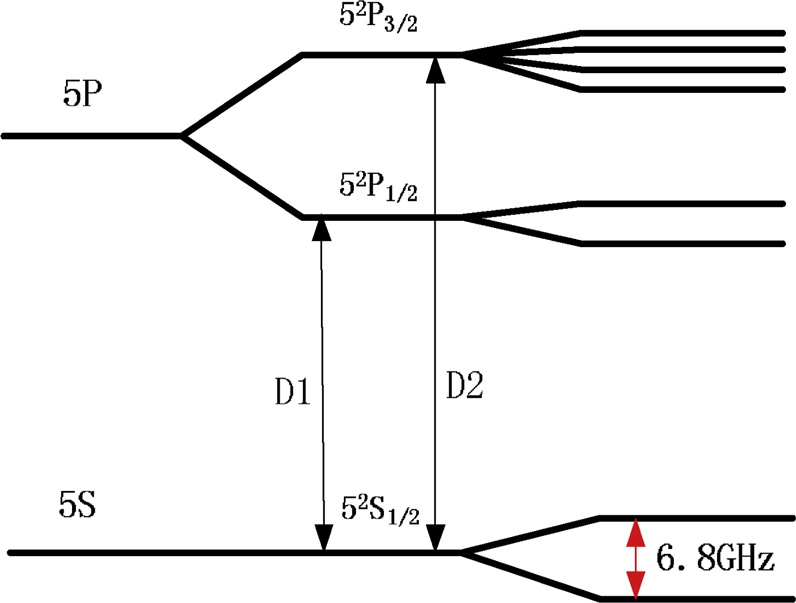
\includegraphics[width=0.5\textwidth]{Images/D1 & D2.png} 
    \caption{Energy level diagram showing the D1 and D2 
    transitions in an alkali metal atom. From \cite{shi2019}}
    \label{fig:energy_levels}
\end{figure}

Collisions between the alkali atoms and other gas molecules
perturb the atomic energy levels, leading to 
collision-induced broadening and a frequency shift. 
If the cell's hermeticity is compromised and atmospheric 
gases leak into the cell, the resulting increase in 
internal pressure ($P$) will cause a detectable width 
broadening and a frequency shift of the Lorentzian profile.
To quantify the gas pressure, the following relations are 
used:
\begin{align}
    \delta \nu &= \delta P \label{eq:delta}
\end{align}
\begin{align}
    \Delta\nu_L &= \gamma P + \gamma_N \label{eq:gamma}
\end{align}

The first equation relates the frequency shift
($\delta\nu$) to the pressure ($P$) through the shift 
rate constant ($\delta$). The second equation links
the pressure to the Lorentzian full width at half maximum
($\Delta \nu_L$), involving the broadening rate constant
$\gamma$ and the natural linewidth $\gamma_N$.

Both $\delta$ and $\gamma$ depend on the specific 
alkali-gas pair and the temperature, with values documented 
in literature 
\cite{pitz2009, pitz2010, andalkar2002, pitz2014, shi2019}.
 Furthermore, the broadening rate $\gamma$ at a temperature
  $T_2$ can be estimated from a known value at $T_1$ using:
\begin{align}
    \gamma(T_2) = \gamma(T_1)\left(\frac{T_1}{T_2}\right)^{\frac{1}{2}}
     \label{eq:gammascale}
\end{align}
Note that the shift constant $\delta$ does not
follow such a simple scaling law due to its more complex 
temperature dependence \cite{pitz2009} 
\subsection{Experimental Proposal}
The spectroscopic framework described above can be directly 
applied to assess the hermeticity of the fabricated vapor 
cells. Here, an experimental procedure similar to the one
followed by Maurice et al.
\cite{maurice2022} is described.

First, the sealed and activated cell is heated to a nominal operating temperature 
$T_\mathrm{op}$ ---chosen so that the alkali vapor pressure 
is sufficient to produce a measurable absorption signal--- 
and held there throughout the measurement campaign using a 
temperature-stabilized mount. Temperature stability is 
critical, since any drift in $T_\mathrm{op}$ would 
introduce a systematic error in the extracted pressure 
through the temperature dependence of $\gamma$ and $\delta$ 
\cite{pitz2009}.

A tunable laser is scanned across the D1 or D2 
absorption line and the transmitted intensity is recorded 
with a photodetector. To avoid power broadening, the probe 
beam intensity is kept well below the saturation intensity 
of the transition. The resulting spectrum is fitted to a 
Voigt profile, from which the Lorentzian width 
$\Delta\nu_L$ and the line center $\nu_0$ are extracted. 
Since the Doppler width depends only on $T_\mathrm{op}$ 
and the atomic mass, the Lorentzian component is 
unambiguously separated. The internal pressure is then 
retrieved using Equations \ref{eq:delta} and \ref{eq:gamma}, evaluated at 
$T_\mathrm{op}$ using literature values of $\gamma$ and 
scaled if necessary via Equation \ref{eq:gammascale}. 
The two estimates of $P$ ---one from the width and one 
from the frequency shift--- serve as a mutual consistency 
check.

Spectra are recorded at regular time intervals: initially 
daily, and subsequently weekly once short-term stability 
has been confirmed. The pressure $P(t)$ is plotted as a 
function of time and, in the case of a small but non-zero 
leak, a linear fit to $P(t)$ yields the leak rate 
$\dot{P}$. If no detectable increase is observed, the 
measurement noise propagated through Equation \ref{eq:gamma} sets 
an upper bound on the leak rate:
\begin{align}
    \sigma_P = \frac{\sigma_{\Delta\nu_L}}
    {\gamma(T_\mathrm{op})}
\end{align}
where $\sigma_{\Delta\nu_L}$ is the uncertainty on the 
fitted Lorentzian width. This bound provides a 
physically meaningful hermeticity statement even in the 
absence of a detectable leak, and allows direct 
comparison with benchmarks from the literature: the 
707-day vacuum integrity demonstrated by 
Artusio-Glimpse et al.~\cite{art2025} using Rydberg 
EIT spectroscopy, and the short-term seal integrity 
inferred from CPT resonance stability by Kobtsev et 
al.~\cite{kobtsev2019} over timescales up to 
$\sim$\SI{1000}{\second}.
